\documentclass[12pt,letterpaper,noanswers]{exam}
\usepackage[usenames,dvipsnames,svgnames,table]{xcolor}
\usepackage[margin=0.9in]{geometry}
\renewcommand{\familydefault}{\sfdefault}
\usepackage{multicol}
\pagestyle{head}
\definecolor{c03}{HTML}{FFDDDD}
\header{AM 108 Class 06}{}{Sept 16: Oscillation}
\runningheadrule
\headrule
\usepackage{graphicx} % more modern
\usepackage{amsmath} 
\usepackage{amssymb} 
\usepackage{hyperref}
\usepackage{tcolorbox}

\begin{document}
 \pdfpageheight 11in 
  \pdfpagewidth 8.5in

\noindent 
\begin{itemize}
    \item There is a problem set due on Friday, but no Check Yourself pre-class assignment.
    \item There is a two question skill check on Friday.  The sample questions for it are below.
    \item Before attending OH, post to \#officehours on Slack (or the Office Hours thread on Piazza) to let your classmates and the course staff know what questions / problems you're bringing to OH.
    \item OH this week: 3-4pm and 7-8:30pm ET Wednesday, 3-4pm (usually 4-5pm) and 8-9:30pm ET Thursday, 3-4pm Friday.  Find the zoom links (and the person staffing the OH) on Canvas.
\end{itemize}

\hrule
\vspace{0.2cm}

\noindent\textbf{Teams}

\begin{multicols}{2}
1. 
\end{multicols}

\noindent \textbf{Teams 3 and 4}: Post screenshots of your work to the course Google Drive today.  Include words, labels, and other short notes that might make those solutions useful to you or your classmates.  Find the link in Canvas (or here: \url{https://drive.google.com/drive/u/0/folders/1GcpwvKHD4tMecpFQ4lNxN_r5Ylj7YHbd})

\vspace{0.2cm}
\hrule
\vspace{0.2cm}


\noindent \textbf{Extra vocabulary / extra facts:}
\begin{tcolorbox}
An oscillator model might be used to represent the \textbf{phase of a single oscillator} (often denoted $\theta$), or the \textbf{phase difference} between two oscillators (often denoted $\phi$).

When the phase difference between two oscillators approaches a constant we call the oscillators \textbf{phase locked}.

When one oscillator is able to phase lock to another, we call the oscillators \textbf{entrained} and call this process of phase locking \textbf{entrainment}.

When the oscillator is not entrained there is \textbf{phase drift} between it and the reference.


\end{tcolorbox}


\vspace{0.2cm}

\hrule
\vspace{0.2cm}

\noindent\textbf{Addressing your questions}

\begin{enumerate}
\itemsep0em
    \item For a 1d system of the form $\dot x = f(x)$, why can't a solution function $x(t)$ cross $x_0$ in an increasing direction at some time, and in a decreasing direction at a later time?
    
\item Consider the system $\dot \theta = \sin\theta - r$.  For $r>1$ but close to $1$, why is the velocity of $\theta$ smaller at $\theta$ values where $\sin\theta$ is close to $1$?
\item For $\dot\theta = \sin\theta - r$ how does the bifurcation diagram connect to the graph of $\sin\theta$ and $r$ vs $\theta$?  How are the fixed points at $r = \pm 1$ different from the fixed points at $r = 0$?
\item For this half-stable fixed point, is it stable from the stable side, and then becomes unstable as you `oscillate'?

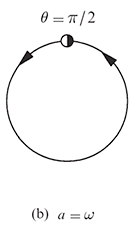
\includegraphics{img/C06book4-3p1.png}

\item When reasoning about the period of an oscillator when close to the bifurcation, will we always use an approximation to the actual function, or will we sometimes use the original function itself?

\item For nondimensionalizing an equation with an angle, why is the angular variable treated as already nondimensional?
\end{enumerate}


\vspace{0.2cm}
\hrule
\vspace{0.2cm}


\noindent\textbf{Skill Check C07 practice}
\begin{questions}
\item (C04) Retake of the C04 skill check question.  This is the one where you need to provide the name of the bifurcation (saddle-node, transcritical, supercritical pitchfork, subcritical pitchfork) when given a bifurcation diagram that includes that bifurcation.
\item Assume the time evolution of the phase difference, $\phi$, between an oscillator and a reference signal is given by the system $\dot\phi = 1.1-\sin\phi$.

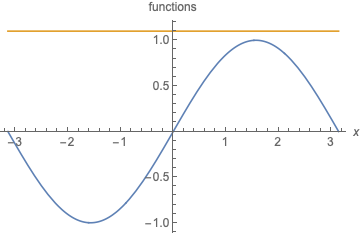
\includegraphics[width=4in]{img/C07-2019-09-18plot2.png}

What is the long term behavior of the phase difference in this system?


\end{questions}




\vspace{0.2cm}

\hrule
\vspace{0.2cm}

\noindent\textbf{Skill Check C07 practice solution}

\begin{questions}
\question See C03 handout.
\question Note that this question requires us to interpret $\phi$ as a phase difference, rather than as the phase of a single oscillator.

If there were an intersection between the orange line and the blue line then the phase difference would approach a fixed value (that you could identify) associated with a stable or half-stable fixed point.

In this picture, though, $\dot\phi = 1.1 - \sin\phi$ and $\sin\phi < 1.1$ for all values of $\phi$.  So $\dot\phi > 0$ for all phase differences, $\phi$.  This means that \textbf{the phase difference is always changing}.  In some sense, it is always increasing ($\dot\phi>0$, after all).  However, when the phase difference passes through $2\pi n$ for $n$ an integer, the oscillator and the reference momentarily have the same phase angle, so if we look at the two oscillators on a circle, one of them will appear to `lap' the other one over and over again. 
\end{questions}

\vspace{0.2cm}

\hrule
\vspace{0.2cm}

\textbf{Questions}


In your post to the \#classactivities Slack channel, provide the number of the question you're posting about.
\begin{questions}
\item (4.1.1) 
(\textbf{team 1}, post a short written explanations of your thinking for this question on the \#classactivities slack channel)

For which values of $a$ does the equation $\dot{\theta} = \sin a\theta$ give a well-defined vector field on the circle?  

For $a = 3$, find and classify all the fixed points and sketch the phase portrait on the circle.  

\emph{You might plot \texttt{Sin[3 $\theta$]} in Mathematica}


\item (4.3.3) For $\dot{\phi} = \mu \sin \phi - \sin 2\phi$:
\begin{parts}
\item (\textbf{Team 2}, post to slack about this if you get to this problem)

Check that the vector field is well-defined on the circle.
\item (\textbf{Team 5}, post to slack about this if you get to this problem)

Draw the qualitatively different phase portraits that exist at different values of $\mu$.
\item (\textbf{Team 6}, post to slack about this if you get to this problem)

Classify the bifurcations that occur as $\mu$ varies.
\item (\textbf{Team 7}, post to slack about this if you get to this problem)

Find the bifurcation values of $\mu$. 
\item (\textbf{Team 2}, post to slack about this if you get to this problem)

Think of $\phi$ as describing the \textbf{phase of a single oscillator}.  For what values of $\mu$ is the system ``oscillating''?
\item (\textbf{Team 5}, post to slack about this if you get to this problem)

Think of $\phi$ as describing the \textbf{phase difference} between an oscillator and a reference.  For what values of $\mu$ is the oscillator entrained (phase-locked) to the reference?
\end{parts}

\emph{You might use Mathematica to find or check the shapes of the bifurcation diagrams}


\end{questions}

\vfill

\eject
\textbf{Answers}.

1: $\sin(a(\theta + 2\pi)) = \sin(a\theta + a2\pi) = \sin(a\theta)\cos(2\pi a)+\cos(a\theta)\sin(2\pi a)$.  When $a$ is an integer, this will lead to $\sin(a(\theta + 2\pi)) = \sin(a\theta)$.  Otherwise, there's a non-zero cosine contribution, which would be a problem.

2a: $\mu\sin(\phi+2\pi) -\sin(2\phi+ 4\pi) = \mu\sin\phi-\sin 2\phi$.  well-defined.  2b: draw for $\mu$ very negative, zero, and very positive.  Then add in an in-between case.  2c: Two subcritical pitchfork bifurcations.  2d: $\mu\sin\phi$ is tangent to $\sin 2\phi$ at the $0$ fixed point when $\mu\phi$ (the linear approximation) is equal to $2\phi$, so when $\mu = 2$.  At $\pi$ the tangency occurs when $\mu = -2$.  So a subcritical pitchfork for $\phi = 0$ and $\mu = 2$ and a subcritical pitchfork for $\phi = \pi$ at $\mu = -2$.  2e: no oscillation ever.  2f: there is always entrainment (there is always a fixed point).

\end{document}